
\subsection{Software Architecture}

As shown in Fig.~\ref{fig:hivewatch}, HiveWatch is designed as a server-side instrumentation layer that sits between an existing federated learning framework and one or more monitoring backends. The FL framework remains fully responsible for client selection, model distribution, local training, and aggregation. HiveWatch is inserted at the server's control flow, where it records events and forwards them to emitter backends without modifying the underlying communication protocol or aggregation algorithm. This separation allows HiveWatch to support APPFL, Flower, NVIDIA FLARE, and custom training loops with no changes to HiveWatch itself.

\begin{figure*}[t]
    \centering
    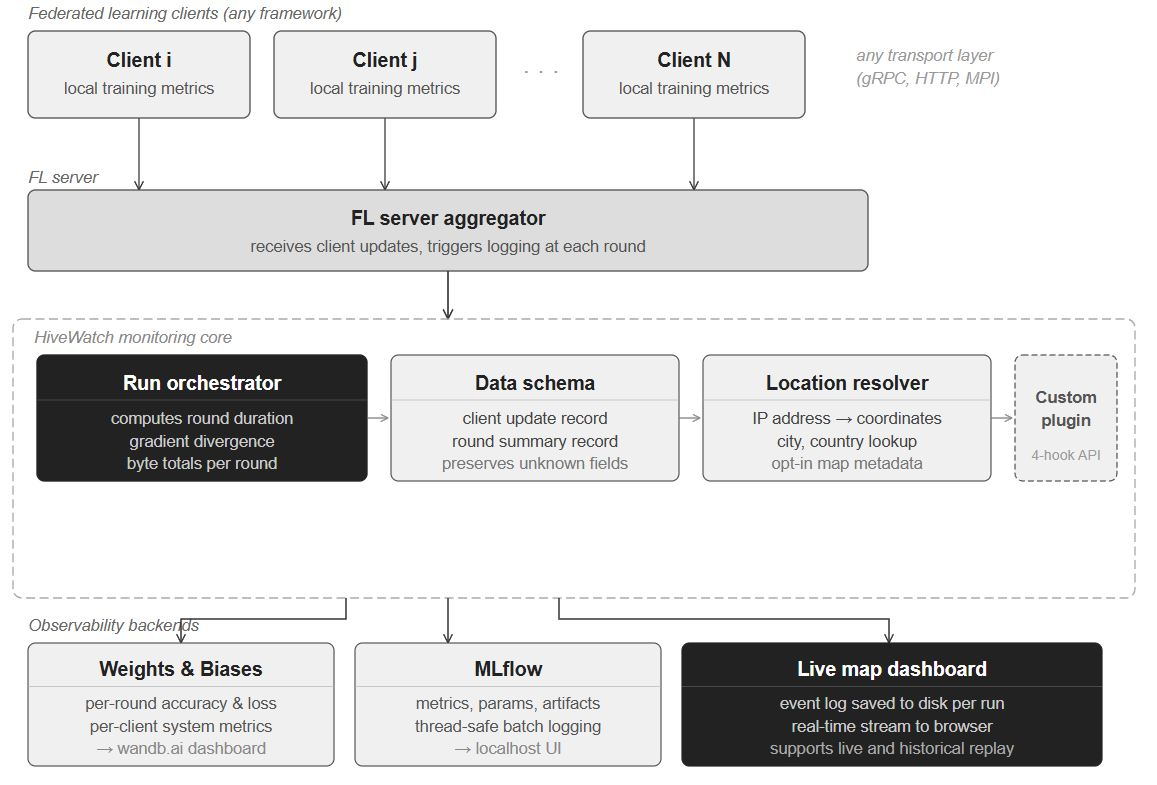
\includegraphics[width=0.9\linewidth]{images/arch.JPG}
    \caption{HiveWatch monitoring framework. The FL server calls the HiveWatch runtime API; events are fanned out to local JSONL artifacts, a map dashboard, MLflow, and Weights \& Biases simultaneously.}
    \label{fig:hivewatch}
\end{figure*}

\subsection{Software Functionalities}

\textbf{Runtime API.}
HiveWatch exposes five primary calls, listed in Table~\ref{tab:api}. During each training round the server marks the round start, records each client update as it arrives, and logs the final round-level summary after aggregation.

\begin{table}[t]
\caption{HiveWatch runtime API.}
\label{tab:api}
\centering
\begin{tabular}{ll}
\toprule
\textbf{Call} & \textbf{When to invoke} \\
\midrule
\texttt{hivewatch.init(\ldots)} & Once at server startup \\
\texttt{round\_start(round)} & Start of each global round \\
\texttt{log\_client\_update(id, **kw)} & Each client result received \\
\texttt{log\_round(round, \ldots)} & After aggregation \\
\texttt{finish()} & Server shutdown \\
\bottomrule
\end{tabular}
\end{table}

\textbf{Event Schema.}
Client updates may include local accuracy, local loss, number of samples, gradient norm and sparsity, bytes sent and received, training wall time, CPU, RAM and GPU utilization, geographic metadata (\texttt{lat}/\texttt{lng}/\texttt{country}), and asynchronous staleness (\texttt{base\_round}). Unknown framework-specific fields are preserved verbatim. Round summaries capture global accuracy and loss, per-round wall time, participation rate, straggler and failure counts, total communication volume, gradient divergence (standard deviation of per-client gradient norms), and aggregation time. Derived quantities — gradient divergence, byte totals, round wall time — are computed once inside HiveWatch and forwarded to every configured backend.

\textbf{Emitter Backends.}
HiveWatch decouples metric collection from metric storage through a pluggable emitter interface. Arbitrary numbers of emitters may be attached simultaneously:

\begin{itemize}[noitemsep]
    \item \textbf{SSEEmitter:} Appends every event to a replayable JSONL event log and rewrites a map-ready \texttt{.map.json} snapshot on every call. Artifacts survive process crashes and enable full post-hoc replay without re-running training.
    \item \textbf{WandbEmitter:} Logs per-client and per-round metrics to Weights \& Biases, using \texttt{wandb.define\_metric()} to align all series on the round axis.
    \item \textbf{MLflowEmitter:} Records metrics, parameters, tags, and model checkpoint artifacts to a local or remote MLflow tracking server. Per-client keys use dot notation to comply with MLflow naming conventions.
\end{itemize}

Custom emitters may be added by implementing four methods: \texttt{on\_init}, \texttt{on\_round}, \texttt{on\_client\_update}, and \texttt{finish}.

\textbf{Map Dashboard.}
The SSEEmitter artifact can be served by the bundled \texttt{hivewatch map run} CLI, which provides a local browser-based dashboard visualising client locations, training status, round progress, straggler markers, and per-client sidebar metadata. Both live runs (streamed via server-sent events) and completed runs (replayed from saved artifacts) are supported.

\subsection{Implementation Notes}

HiveWatch is a pure-Python package (Python~$\geq$~3.8) released under the MIT license. The core package has no mandatory third-party dependencies beyond the standard library. Weights~\&~Biases and MLflow support are optional extras installed via \texttt{pip install hivewatch[wandb]}, \texttt{pip install hivewatch[mlflow]}, or \texttt{pip install hivewatch[all]}. Internal bookkeeping uses a single \texttt{threading.Lock} so that \texttt{log\_client\_update()} is safe to call from concurrent server threads. The package ships the map dashboard HTML file as a package data asset; no build step or web bundler is required.
